\clearpage
\makeatletter
\efloat@restorefloats
\makeatother


\begin{appendix}
\hypertarget{sa-confirming-the-five-factor-solution-obtained-using-minimum-residual-extraction-method}{%
\section{SA: Confirming the five factor solution obtained using minimum
residual extraction
method}\label{sa-confirming-the-five-factor-solution-obtained-using-minimum-residual-extraction-method}}

\begin{center}
\begin{ThreePartTable}

\begin{TableNotes}[para]
\normalsize{\textit{Note.} Only loading higher than .30 is reported}
\end{TableNotes}

\begin{longtable}{llllllll}\noalign{\getlongtablewidth\global\LTcapwidth=\longtablewidth}
\caption{\label{tab:MinResTab}Factor loadings and communality of the retained items(Minmum Residual)}\\
\toprule
item & \multicolumn{1}{c}{MR1} & \multicolumn{1}{c}{MR2} & \multicolumn{1}{c}{MR3} & \multicolumn{1}{c}{MR4} & \multicolumn{1}{c}{MR5} & \multicolumn{1}{c}{Communality} & \multicolumn{1}{c}{Uniqueness}\\
\midrule
\endfirsthead
\caption*{\normalfont{Table \ref{tab:MinResTab} continued}}\\
\toprule
item & \multicolumn{1}{c}{MR1} & \multicolumn{1}{c}{MR2} & \multicolumn{1}{c}{MR3} & \multicolumn{1}{c}{MR4} & \multicolumn{1}{c}{MR5} & \multicolumn{1}{c}{Communality} & \multicolumn{1}{c}{Uniqueness}\\
\midrule
\endhead
item16 & 1 &  &  &  &  & 0.996 & 0.004\\
item36 & 0.94 &  &  &  &  & 0.897 & 0.103\\
item17 & 0.8 &  &  &  &  & 0.658 & 0.342\\
item11 &  & 0.79 &  &  &  & 0.642 & 0.358\\
item10 &  & 0.76 &  &  &  & 0.592 & 0.408\\
item12 &  & 0.65 &  &  &  & 0.465 & 0.535\\
item7 &  & 0.5 &  &  &  & 0.267 & 0.733\\
item8 &  & -0.49 &  &  &  & 0.252 & 0.748\\
item9 &  & 0.32 &  &  &  & 0.113 & 0.887\\
item27 &  &  & 0.8 &  &  & 0.659 & 0.341\\
item3 &  &  & 0.8 &  &  & 0.683 & 0.317\\
item40 &  &  & 0.65 &  &  & 0.464 & 0.536\\
item30 &  &  & 0.45 &  &  & 0.353 & 0.647\\
item41 &  &  & 0.36 &  &  & 0.329 & 0.671\\
item33 &  &  &  & 0.74 &  & 0.555 & 0.445\\
item32 &  &  &  & 0.73 &  & 0.623 & 0.377\\
item35 &  &  &  & 0.66 &  & 0.455 & 0.545\\
item37 &  &  &  & -0.39 &  & 0.175 & 0.825\\
item38 &  &  &  & 0.38 &  & 0.178 & 0.822\\
item46 &  &  &  &  & 0.6 & 0.422 & 0.578\\
item45 &  &  &  &  & 0.59 & 0.374 & 0.626\\
item25 &  &  &  &  & 0.41 & 0.193 & 0.807\\
item4 &  &  &  &  & 0.41 & 0.219 & 0.781\\
item1 &  &  &  &  & 0.4 & 0.17 & 0.83\\
item26 &  &  &  &  & 0.35 & 0.165 & 0.835\\
\% of Variance & 0.1 & 0.1 & 0.09 & 0.08 & 0.06 &  & \\
\bottomrule
\addlinespace
\insertTableNotes
\end{longtable}

\end{ThreePartTable}
\end{center}

\hypertarget{sa-factor-analysis-with-six-factors}{%
\section{SA: Factor analysis with six
factors}\label{sa-factor-analysis-with-six-factors}}

\begin{center}
\begin{ThreePartTable}

\begin{TableNotes}[para]
\normalsize{\textit{Note.} Only loading higher than .30 is reported}
\end{TableNotes}

\begin{longtable}{lllllllll}\noalign{\getlongtablewidth\global\LTcapwidth=\longtablewidth}
\caption{\label{tab:sixFacTab}Factor loadings and communality of the retained items(six factor)}\\
\toprule
item & \multicolumn{1}{c}{PA1} & \multicolumn{1}{c}{PA4} & \multicolumn{1}{c}{PA2} & \multicolumn{1}{c}{PA3} & \multicolumn{1}{c}{PA5} & \multicolumn{1}{c}{PA6} & \multicolumn{1}{c}{Communality} & \multicolumn{1}{c}{Uniqueness}\\
\midrule
\endfirsthead
\caption*{\normalfont{Table \ref{tab:sixFacTab} continued}}\\
\toprule
item & \multicolumn{1}{c}{PA1} & \multicolumn{1}{c}{PA4} & \multicolumn{1}{c}{PA2} & \multicolumn{1}{c}{PA3} & \multicolumn{1}{c}{PA5} & \multicolumn{1}{c}{PA6} & \multicolumn{1}{c}{Communality} & \multicolumn{1}{c}{Uniqueness}\\
\midrule
\endhead
item19 & 1.78 &  &  &  &  &  & 3.318 & -2.318\\
item5 &  &  &  &  &  &  & 0.11 & 0.89\\
item16 &  & 1 &  &  &  &  & 1.004 & -0.004\\
item36 &  & 0.91 &  &  &  &  & 0.86 & 0.14\\
item17 &  & 0.81 &  &  &  &  & 0.691 & 0.309\\
item11 &  &  & 0.83 &  &  &  & 0.71 & 0.29\\
item10 &  &  & 0.79 &  &  &  & 0.638 & 0.362\\
item12 &  &  & 0.63 &  &  &  & 0.465 & 0.535\\
item8 &  &  & -0.5 &  &  &  & 0.269 & 0.731\\
item7 &  &  & 0.47 &  &  &  & 0.268 & 0.732\\
item9 &  &  & 0.32 &  &  &  & 0.163 & 0.837\\
item33 &  &  &  & 0.83 &  &  & 0.698 & 0.302\\
item32 &  &  &  & 0.75 &  &  & 0.666 & 0.334\\
item35 &  &  &  & 0.64 &  &  & 0.446 & 0.554\\
item31 &  &  &  & 0.48 &  &  & 0.331 & 0.669\\
item38 &  &  &  & 0.39 &  &  & 0.191 & 0.809\\
item37 &  &  &  & -0.35 &  &  & 0.153 & 0.847\\
item3 &  &  &  &  & 0.85 &  & 0.748 & 0.252\\
item27 &  &  &  &  & 0.8 &  & 0.644 & 0.356\\
item40 &  &  &  &  & 0.68 &  & 0.507 & 0.493\\
item46 &  &  &  &  &  & 0.6 & 0.431 & 0.569\\
item45 &  &  &  &  &  & 0.56 & 0.341 & 0.659\\
item4 &  &  &  &  &  & 0.43 & 0.265 & 0.735\\
item25 &  &  &  &  &  & 0.4 & 0.178 & 0.822\\
item1 &  &  &  &  &  & 0.36 & 0.142 & 0.858\\
item26 &  &  &  &  &  & 0.36 & 0.173 & 0.827\\
item13 &  &  &  &  &  &  & 0.087 & 0.913\\
item29 &  &  &  &  &  &  & 0.108 & 0.892\\
\% of Variance & 0.12 & 0.09 & 0.09 & 0.08 & 0.07 & 0.06 &  & \\
\bottomrule
\addlinespace
\insertTableNotes
\end{longtable}

\end{ThreePartTable}
\end{center}

\hypertarget{sa-factor-analysis-with-unmerged-response-option}{%
\section{SA: Factor Analysis with Unmerged Response
Option}\label{sa-factor-analysis-with-unmerged-response-option}}

Table @ref(tab:tabDesAppB) summarizes the univariate descriptive
statistics for the 48 items with un-merged options. Some of the items
were skewed with high Kurtosis values. Our data violated both univariate
normality (Shapiro-Wilk statistics) and multivariate normality
assumptions {[}Marida's test{]}. Multivariate skew was = 494.70 (p
\textless0.001) and multivariate kurtosis was = 2,705.00 (p
\textless0.001). Due to these violations and ordinal nature of the
response data polychoric correlations over Pearson's correlations was
chosen. Sampling adequacy was checked using Kaiser-Meyer-Olkin (KMO)
measures of sampling adequacy. The overall KMO vale for 48 items was
0.65 which was above the cutoff value (.50) indicating a mediocre
sample. Bartlett's test of sphericity, \(\chi^2\) (1128) = 5515.20, p
\textless{} .001 indicated the correlations between items are adequate
for the EFA. However only 4.34\% of the inter-item correlation
coefficients were greater than .30. The absolute value of inter-item
correlation ranged between .00 to .96.Figure @ref(fig:figCorAppB)
depicts the correlation matrix. For un-merged response option Horn's
parallel analysis with 500 iterations indicated a five-factor solution.
However, Scree plot and the MAP method suggested 6-factor solution.
five-factor solution . As a result, we tested both five-factor and
six-factor solutions. The six factor solution yielded a factor with only
two salient loading (Table @ref(tab:EFAsix). Thus we reject the six
factor solution. The five factor solution retained 24 items (Table
@ref(tab:EFATableAppB)). However the factors are less interpretable in
terms of common theme. Thus we reject the five factor solution.

\begin{center}
\begin{ThreePartTable}

\begin{TableNotes}[para]
\normalsize{\textit{Note.} *p<.001}
\end{TableNotes}

\begin{longtable}{lllllll}\noalign{\getlongtablewidth\global\LTcapwidth=\longtablewidth}
\caption{\label{tab:tabDesAppB}Descriptive Statistics for Unmerged response options}\\
\toprule
 & \multicolumn{1}{c}{Mean} & \multicolumn{1}{c}{SD} & \multicolumn{1}{c}{Skew} & \multicolumn{1}{c}{Kurtosis} & \multicolumn{1}{c}{Shapiro-Wilk Statistics} & \multicolumn{1}{c}{Item-Total Correlation}\\
\midrule
\endfirsthead
\caption*{\normalfont{Table \ref{tab:tabDesAppB} continued}}\\
\toprule
 & \multicolumn{1}{c}{Mean} & \multicolumn{1}{c}{SD} & \multicolumn{1}{c}{Skew} & \multicolumn{1}{c}{Kurtosis} & \multicolumn{1}{c}{Shapiro-Wilk Statistics} & \multicolumn{1}{c}{Item-Total Correlation}\\
\midrule
\endhead
Item1 & 2.16 & 1.51 & 0.49 & -0.86 & 0.90* & .21\\
Item2 & 2.76 & 1.75 & -0.10 & -1.42 & 0.88* & .20\\
Item3 & 3.34 & 1.43 & -0.58 & -0.77 & 0.88* & .18\\
Item4 & 1.30 & 1.31 & 1.93 & 2.92 & 0.62* & .32\\
Item5 & 3.95 & 1.56 & -1.42 & 0.75 & 0.70* & .19\\
Item6 & 2.70 & 1.66 & 0.02 & -1.33 & 0.90* & .18\\
Item7 & 2.23 & 1.28 & 0.60 & -0.59 & 0.89* & .18\\
Item8 & 2.95 & 1.24 & -0.19 & -0.70 & 0.93* & -.07\\
Item9 & 2.92 & 1.09 & -0.37 & 0.11 & 0.91* & .14\\
Item10 & 2.73 & 1.07 & -0.03 & -0.52 & 0.92* & .27\\
Item11 & 2.17 & 0.93 & 0.44 & 0.20 & 0.89* & .25\\
Item12 & 2.34 & 1.26 & 0.46 & -0.58 & 0.91* & .24\\
Item13 & 2.71 & 1.49 & 0.14 & -1.29 & 0.89* & .28\\
Item14 & 2.11 & 1.34 & 0.68 & -0.78 & 0.84* & .24\\
Item15 & 3.26 & 1.11 & -0.34 & -0.21 & 0.91* & .11\\
Item16 & 1.46 & 1.31 & 1.71 & 1.90 & 0.65* & .33\\
Item17 & 1.43 & 1.30 & 1.76 & 2.12 & 0.64* & .30\\
Item18 & 0.92 & 0.67 & 2.00 & 9.41 & 0.62* & .32\\
Item19 & 0.85 & 0.56 & 1.71 & 10.74 & 0.55* & .34\\
Item20 & 0.83 & 0.54 & 1.76 & 13.92 & 0.53* & .31\\
Item21 & 0.94 & 0.75 & 2.46 & 10.66 & 0.58* & .27\\
Item22 & 3.57 & 1.08 & -0.72 & 0.08 & 0.88* & .19\\
Item23 & 2.53 & 1.31 & 0.22 & -0.91 & 0.92* & .11\\
Item24 & 4.13 & 1.01 & -1.39 & 2.01 & 0.78* & .19\\
Item25 & 2.57 & 1.43 & 0.22 & -1.23 & 0.88* & .17\\
Item26 & 2.23 & 1.30 & 0.59 & -0.63 & 0.88* & .16\\
Item27 & 3.78 & 1.34 & -1.01 & 0.08 & 0.82* & .18\\
Item28 & 3.75 & 1.16 & -0.78 & -0.10 & 0.86* & .01\\
Item29 & 2.38 & 1.40 & 0.20 & -1.04 & 0.92* & .11\\
Item30 & 0.94 & 1.42 & 1.66 & 1.69 & 0.68* & .24\\
Item31 & 2.91 & 1.76 & -0.24 & -1.41 & 0.87* & .45\\
Item32 & 3.49 & 1.76 & -0.71 & -1.06 & 0.78* & .43\\
Item33 & 3.56 & 1.75 & -0.79 & -0.95 & 0.77* & .32\\
Item34 & 3.30 & 2.00 & -0.54 & -1.50 & 0.74* & .34\\
Item35 & 3.80 & 1.79 & -1.07 & -0.59 & 0.67* & .24\\
Item36 & 1.36 & 1.38 & 1.75 & 2.05 & 0.65* & .38\\
Item37 & 1.30 & 0.94 & 2.79 & 7.65 & 0.48* & -.01\\
Item38 & 4.27 & 1.18 & -2.07 & 4.01 & 0.65* & .23\\
Item39 & 1.94 & 1.01 & 0.85 & 0.61 & 0.86* & .05\\
Item40 & 2.13 & 1.24 & 0.56 & -0.54 & 0.89* & .16\\
Item41 & 0.87 & 1.08 & 1.68 & 2.74 & 0.73* & .21\\
Item42 & 3.90 & 1.55 & -1.15 & -0.12 & 0.72* & .17\\
Item43 & 1.59 & 1.23 & 1.59 & 1.70 & 0.69* & .22\\
Item44 & 3.46 & 1.41 & -0.92 & -0.01 & 0.86* & .38\\
Item45 & 2.04 & 1.66 & 0.46 & -1.12 & 0.87* & .29\\
Item46 & 1.57 & 1.40 & 0.97 & -0.07 & 0.82* & .38\\
Item47 & 2.07 & 1.23 & 0.59 & -0.42 & 0.89* & .34\\
Item48 & 2.57 & 1.30 & 0.14 & -0.74 & 0.93* & .31\\
\bottomrule
\addlinespace
\insertTableNotes
\end{longtable}

\end{ThreePartTable}
\end{center}

\begin{figure}
\centering
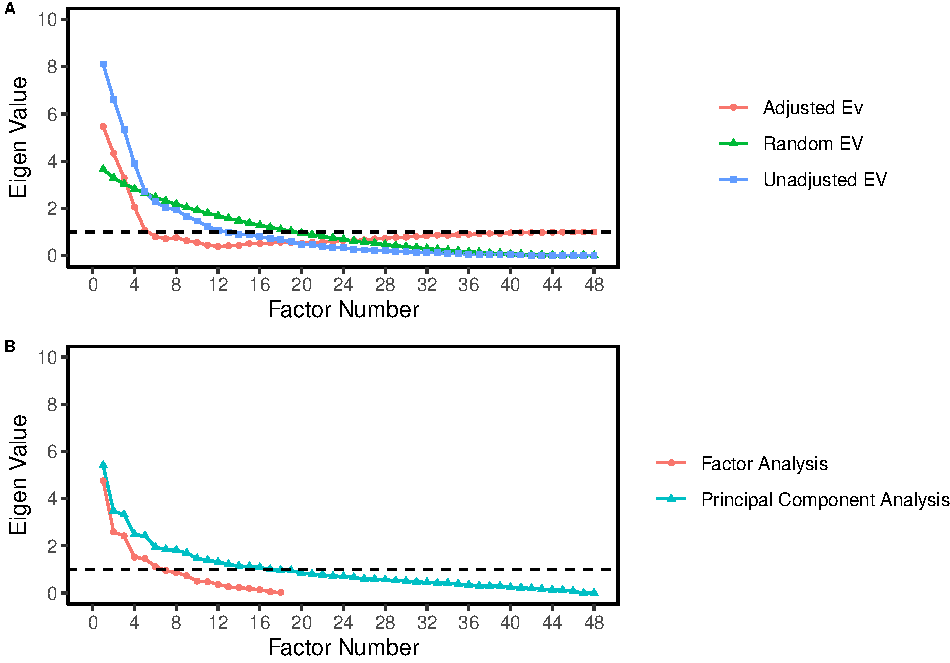
\includegraphics{manuscript_files/figure-latex/facIdFigAppB-1.pdf}
\caption{(\#fig:facIdFigAppB)Factor Identification (A) Parallel analysis
(B) Scree Plot {[}Unmerged response options{]}}
\end{figure}

\begin{center}
\begin{ThreePartTable}

\begin{TableNotes}[para]
\normalsize{\textit{Note.} Only loading higher than .30 is reported}
\end{TableNotes}

\begin{longtable}{llllllll}\noalign{\getlongtablewidth\global\LTcapwidth=\longtablewidth}
\caption{\label{tab:EFATableAppB}Factor loadings and communality of the retained items in five factor solution [Unmerged Responses]}\\
\toprule
item & \multicolumn{1}{c}{PA1} & \multicolumn{1}{c}{PA2} & \multicolumn{1}{c}{PA5} & \multicolumn{1}{c}{PA3} & \multicolumn{1}{c}{PA4} & \multicolumn{1}{c}{Communality} & \multicolumn{1}{c}{Uniqueness}\\
\midrule
\endfirsthead
\caption*{\normalfont{Table \ref{tab:EFATableAppB} continued}}\\
\toprule
item & \multicolumn{1}{c}{PA1} & \multicolumn{1}{c}{PA2} & \multicolumn{1}{c}{PA5} & \multicolumn{1}{c}{PA3} & \multicolumn{1}{c}{PA4} & \multicolumn{1}{c}{Communality} & \multicolumn{1}{c}{Uniqueness}\\
\midrule
\endhead
item19 & 0.99 &  &  &  &  & 1.007 & -0.007\\
item20 & 0.91 &  &  &  &  & 0.874 & 0.126\\
item18 & 0.82 &  &  &  &  & 0.711 & 0.289\\
item21 & 0.8 &  &  &  &  & 0.683 & 0.317\\
item4 & 0.47 &  &  &  &  & 0.25 & 0.75\\
item11 &  & 0.83 &  &  &  & 0.687 & 0.313\\
item10 &  & 0.81 &  &  &  & 0.67 & 0.33\\
item12 &  & 0.56 &  &  &  & 0.371 & 0.629\\
item8 &  & -0.44 &  &  &  & 0.206 & 0.794\\
item7 &  & 0.42 &  &  &  & 0.226 & 0.774\\
item9 &  & 0.33 &  &  &  & 0.115 & 0.885\\
item16 &  &  & 0.95 &  &  & 0.946 & 0.054\\
item17 &  &  & 0.74 &  &  & 0.595 & 0.405\\
item36 & 0.3 &  & 0.73 &  &  & 0.653 & 0.347\\
item3 &  &  &  & 0.85 &  & 0.746 & 0.254\\
item27 &  &  &  & 0.78 &  & 0.624 & 0.376\\
item40 &  &  &  & 0.71 &  & 0.512 & 0.488\\
item35 &  &  &  &  & 0.58 & 0.351 & 0.649\\
item48 &  &  &  &  & 0.57 & 0.354 & 0.646\\
item33 &  &  &  &  & 0.55 & 0.32 & 0.68\\
item47 &  &  &  &  & 0.52 & 0.294 & 0.706\\
item44 &  &  &  &  & 0.45 & 0.216 & 0.784\\
item31 &  &  &  &  & 0.41 & 0.206 & 0.794\\
item38 &  &  &  &  & 0.33 & 0.129 & 0.871\\
\% of Variance & 0.15 & 0.09 & 0.09 & 0.08 & 0.08 &  & \\
\bottomrule
\addlinespace
\insertTableNotes
\end{longtable}

\end{ThreePartTable}
\end{center}

\begin{center}
\begin{ThreePartTable}

\begin{TableNotes}[para]
\normalsize{\textit{Note.} Only loading higher than .30 is reported}
\end{TableNotes}

\begin{longtable}{lllllllll}\noalign{\getlongtablewidth\global\LTcapwidth=\longtablewidth}
\caption{\label{tab:EFAsix}Factor loadings and communality of the retained items in six factor solution [Unmerged Responses]}\\
\toprule
item & \multicolumn{1}{c}{PA1} & \multicolumn{1}{c}{PA2} & \multicolumn{1}{c}{PA3} & \multicolumn{1}{c}{PA4} & \multicolumn{1}{c}{PA6} & \multicolumn{1}{c}{PA5} & \multicolumn{1}{c}{Communality} & \multicolumn{1}{c}{Uniqueness}\\
\midrule
\endfirsthead
\caption*{\normalfont{Table \ref{tab:EFAsix} continued}}\\
\toprule
item & \multicolumn{1}{c}{PA1} & \multicolumn{1}{c}{PA2} & \multicolumn{1}{c}{PA3} & \multicolumn{1}{c}{PA4} & \multicolumn{1}{c}{PA6} & \multicolumn{1}{c}{PA5} & \multicolumn{1}{c}{Communality} & \multicolumn{1}{c}{Uniqueness}\\
\midrule
\endhead
item19 & 0.98 &  &  &  &  &  & 0.995 & 0.005\\
item20 & 0.92 &  &  &  &  &  & 0.904 & 0.096\\
item21 & 0.79 &  &  &  &  &  & 0.666 & 0.334\\
item4 & 0.49 &  &  &  &  &  & 0.296 & 0.704\\
item43 & 0.32 &  &  &  &  & 0.31 & 0.282 & 0.718\\
item10 &  & 0.81 &  &  &  &  & 0.67 & 0.33\\
item11 &  & 0.81 &  &  &  &  & 0.668 & 0.332\\
item12 &  & 0.58 &  &  &  &  & 0.408 & 0.592\\
item8 &  & -0.45 &  &  &  &  & 0.218 & 0.782\\
item7 &  & 0.42 &  &  &  &  & 0.229 & 0.771\\
item9 &  & 0.33 &  &  &  &  & 0.115 & 0.885\\
item3 &  &  & 0.85 &  &  &  & 0.731 & 0.269\\
item27 &  &  & 0.77 &  &  &  & 0.606 & 0.394\\
item40 &  &  & 0.72 &  &  &  & 0.533 & 0.467\\
item35 &  &  &  & 0.64 &  &  & 0.426 & 0.574\\
item33 &  &  &  & 0.62 &  &  & 0.413 & 0.587\\
item48 &  &  &  & 0.52 &  &  & 0.305 & 0.695\\
item47 &  &  &  & 0.48 &  &  & 0.259 & 0.741\\
item31 &  &  &  & 0.39 &  &  & 0.206 & 0.794\\
item38 &  &  &  & 0.32 &  &  & 0.18 & 0.82\\
item17 &  &  &  &  & 0.85 &  & 0.786 & 0.214\\
item16 &  &  &  &  & 0.78 &  & 0.681 & 0.319\\
item13 &  &  &  &  &  & 0.57 & 0.336 & 0.664\\
item14 &  &  &  &  &  & 0.5 & 0.356 & 0.644\\
item15 &  &  &  &  &  & 0.48 & 0.277 & 0.723\\
item42 &  &  &  &  &  & 0.37 & 0.168 & 0.832\\
item26 &  &  &  &  &  &  & 0.064 & 0.936\\
\% of Variance & 0.11 & 0.08 & 0.07 & 0.06 & 0.06 & 0.05 &  & \\
\bottomrule
\addlinespace
\insertTableNotes
\end{longtable}

\end{ThreePartTable}
\end{center}

\hypertarget{items-retained-in-the-five-factor-solution-unmerged-responses}{%
\section{Items Retained in the Five Factor Solution {[}Unmerged
Responses{]}}\label{items-retained-in-the-five-factor-solution-unmerged-responses}}

\begin{longtable}[]{@{}
  >{\raggedright\arraybackslash}p{(\columnwidth - 0\tabcolsep) * \real{1.00}}@{}}
\toprule
\begin{minipage}[b]{\linewidth}\raggedright
\textbf{Five Factor Solution {[}Unmerged Responses{]} (24 Items)}
\end{minipage} \\
\midrule
\endhead
\textbf{F1} \\
I use light therapy applying a blue light box. \\
I use light therapy applying a light visor. \\
I use light therapy applying a white light box. \\
I use light therapy applying another form of light device. \\
I use an alarm with a dawn simulation light. \\
\textbf{F2} \\
I spend more than 3 hours per day (in total) outside. \\
I spend between 1 and 3 hours per day (in total) outside. \\
I spend as much time outside as possible. \\
I spend 30 minutes or less per day (in total) outside. \\
I go for a walk or exercise outside within 2 hours after waking up. \\
I spend between 30 minutes and 1 hour per day (in total) outside. \\
\textbf{F3} \\
I look at my mobile phone screen immediately after waking up. \\
I use my mobile phone within 1 hour before attempting to fall asleep. \\
I check my phone when I wake up at night. \\
\textbf{F4} \\
I use a blue-filter app on my computer screen within 1 hour before
attempting to fall asleep. \\
I seek out knowledge on how to improve my light exposure. \\
I dim my computer screen within 1 hour before attempting to fall
asleep. \\
I discuss the effects of light on my body with other people. \\
I modify my light environment to match my current needs. \\
I dim my room light within 1 hour before attempting to fall asleep. \\
I use as little light as possible when I get up during the night. \\
\textbf{F5} \\
I wear blue-filtering, orange-tinted, and/or red-tinted glasses indoors
during the day. \\
I wear blue-filtering, orange-tinted, and/or red-tinted glasses outdoors
during the day. \\
I wear blue-filtering, orange-tinted, and/or red-tinted glasses within 1
hour before attempting to fall asleep. \\
\bottomrule
\end{longtable}

\hypertarget{geographic-locations-of-survey-participants}{%
\section{Geographic Locations of Survey
Participants}\label{geographic-locations-of-survey-participants}}

\begin{table}

\caption{(\#tab:TzTable)Geographical Location}
\centering
\resizebox{\linewidth}{!}{
\begin{tabular}[t]{ll}
\toprule
 & N = 690\\
\midrule
Time zone - Country & \\
\hspace{1em}United States - America/New\_York (UTC -04:00) & 63 (9.1\%)\\
\hspace{1em}United Kingdom - Europe/London (UTC) & 57 (8.3\%)\\
\hspace{1em}Germany - Europe/Berlin (UTC +01:00) & 53 (7.7\%)\\
\hspace{1em}India - Asia/Kolkata (UTC +05:30) & 38 (5.5\%)\\
\addlinespace
\hspace{1em}United States - America/Los\_Angeles (UTC -07:00) & 37 (5.4\%)\\
\hspace{1em}United States - America/Chicago (UTC -05:00) & 30 (4.3\%)\\
\hspace{1em}France - Europe/Paris (UTC +01:00) & 22 (3.2\%)\\
\hspace{1em}Switzerland - Europe/Zurich (UTC +01:00) & 21 (3.0\%)\\
\hspace{1em}Brazil - America/Sao\_Paulo (UTC -03:00) & 19 (2.8\%)\\
\addlinespace
\hspace{1em}Netherlands - Europe/Amsterdam (UTC +01:00) & 19 (2.8\%)\\
\hspace{1em}Canada - America/Toronto (UTC -04:00) & 16 (2.3\%)\\
\hspace{1em}Poland - Europe/Warsaw (UTC +01:00) & 15 (2.2\%)\\
\hspace{1em}Canada - America/Edmonton (UTC -06:00) & 14 (2.0\%)\\
\hspace{1em}Finland - Europe/Helsinki (UTC +02:00) & 9 (1.3\%)\\
\addlinespace
\hspace{1em}Indonesia - Asia/Jakarta (UTC +07:00) & 9 (1.3\%)\\
\hspace{1em}Italy - Europe/Rome (UTC +01:00) & 9 (1.3\%)\\
\hspace{1em}Chile - America/Santiago (UTC -03:00) & 8 (1.2\%)\\
\hspace{1em}Russian Federation - Europe/Moscow (UTC +03:00) & 8 (1.2\%)\\
\hspace{1em}China - Asia/Shanghai (UTC +08:00) & 7 (1.0\%)\\
\addlinespace
\hspace{1em}Malaysia - Asia/Kuala\_Lumpur (UTC +08:00) & 7 (1.0\%)\\
\hspace{1em}Spain - Europe/Madrid (UTC +01:00) & 7 (1.0\%)\\
\hspace{1em}United States - America/Phoenix (UTC -07:00) & 7 (1.0\%)\\
\hspace{1em}Canada - America/Vancouver (UTC -07:00) & 6 (0.9\%)\\
\hspace{1em}New Zealand - Pacific/Auckland (UTC +13:00) & 6 (0.9\%)\\
\addlinespace
\hspace{1em}Philippines - Asia/Manila (UTC +08:00) & 6 (0.9\%)\\
\hspace{1em}Turkey - Europe/Istanbul (UTC +03:00) & 6 (0.9\%)\\
\hspace{1em}United States - America/Denver (UTC -06:00) & 6 (0.9\%)\\
\hspace{1em}United States - America/Detroit (UTC -04:00) & 6 (0.9\%)\\
\hspace{1em}Argentina - America/Argentina/Buenos\_Aires (UTC -03:00) & 5 (0.7\%)\\
\addlinespace
\hspace{1em}Australia - Australia/Melbourne (UTC +11:00) & 5 (0.7\%)\\
\hspace{1em}Ireland - Europe/Dublin (UTC) & 5 (0.7\%)\\
\hspace{1em}Lithuania - Europe/Vilnius (UTC +02:00) & 5 (0.7\%)\\
\hspace{1em}South Africa - Africa/Johannesburg (UTC +02:00) & 5 (0.7\%)\\
\hspace{1em}Australia - Australia/Brisbane (UTC +10:00) & 4 (0.6\%)\\
\addlinespace
\hspace{1em}Belgium - Europe/Brussels (UTC +01:00) & 4 (0.6\%)\\
\hspace{1em}Israel - Asia/Jerusalem (UTC +02:00) & 4 (0.6\%)\\
\hspace{1em}Sweden - Europe/Stockholm (UTC +01:00) & 4 (0.6\%)\\
\hspace{1em}United States - America/Boise (UTC -06:00) & 4 (0.6\%)\\
\hspace{1em}Czech Republic - Europe/Prague (UTC +01:00) & 3 (0.4\%)\\
\addlinespace
\hspace{1em}Denmark - Europe/Copenhagen (UTC +01:00) & 3 (0.4\%)\\
\hspace{1em}Germany - Europe/Busingen (UTC +01:00) & 3 (0.4\%)\\
\hspace{1em}Greece - Europe/Athens (UTC +02:00) & 3 (0.4\%)\\
\hspace{1em}Iran & 3 (0.4\%)\\
\hspace{1em}Japan - Asia/Tokyo (UTC +09:00) & 3 (0.4\%)\\
\addlinespace
\hspace{1em}Norway - Europe/Oslo (UTC +01:00) & 3 (0.4\%)\\
\hspace{1em}Romania - Europe/Bucharest (UTC +02:00) & 3 (0.4\%)\\
\hspace{1em}Serbia - Europe/Belgrade (UTC +01:00) & 3 (0.4\%)\\
\hspace{1em}Slovenia - Europe/Ljubljana (UTC +01:00) & 3 (0.4\%)\\
\hspace{1em}Taiwan & 3 (0.4\%)\\
\addlinespace
\hspace{1em}United States - America/Anchorage (UTC -08:00) & 3 (0.4\%)\\
\hspace{1em}United States - America/Indiana/Indianapolis (UTC -04:00) & 3 (0.4\%)\\
\hspace{1em}United States - America/Kentucky/Louisville (UTC -04:00) & 3 (0.4\%)\\
\hspace{1em}Argentina - America/Argentina/Cordoba (UTC -03:00) & 2 (0.3\%)\\
\hspace{1em}Australia - Australia/Adelaide (UTC +10:30) & 2 (0.3\%)\\
\addlinespace
\hspace{1em}Australia - Australia/Perth (UTC +08:00) & 2 (0.3\%)\\
\hspace{1em}Australia - Australia/Sydney (UTC +11:00) & 2 (0.3\%)\\
\hspace{1em}Brazil - America/Araguaina (UTC -03:00) & 2 (0.3\%)\\
\hspace{1em}Brazil - America/Bahia (UTC -03:00) & 2 (0.3\%)\\
\hspace{1em}Canada - America/Moncton (UTC -03:00) & 2 (0.3\%)\\
\addlinespace
\hspace{1em}Colombia - America/Bogota (UTC -05:00) & 2 (0.3\%)\\
\hspace{1em}Costa Rica - America/Costa\_Rica (UTC -06:00) & 2 (0.3\%)\\
\hspace{1em}Croatia - Europe/Zagreb (UTC +01:00) & 2 (0.3\%)\\
\hspace{1em}Ecuador - America/Guayaquil (UTC -05:00) & 2 (0.3\%)\\
\hspace{1em}Estonia - Europe/Tallinn (UTC +02:00) & 2 (0.3\%)\\
\addlinespace
\hspace{1em}Hong Kong - Asia/Hong\_Kong (UTC +08:00) & 2 (0.3\%)\\
\hspace{1em}Hungary - Europe/Budapest (UTC +01:00) & 2 (0.3\%)\\
\hspace{1em}Jordan - Asia/Amman (UTC +03:00) & 2 (0.3\%)\\
\hspace{1em}Latvia - Europe/Riga (UTC +02:00) & 2 (0.3\%)\\
\hspace{1em}Malaysia - Asia/Kuching (UTC +08:00) & 2 (0.3\%)\\
\addlinespace
\hspace{1em}Mexico - America/Mexico\_City (UTC -06:00) & 2 (0.3\%)\\
\hspace{1em}Nepal - Asia/Kathmandu (UTC +05:45) & 2 (0.3\%)\\
\hspace{1em}Portugal - Europe/Lisbon (UTC) & 2 (0.3\%)\\
\hspace{1em}Slovakia - Europe/Bratislava (UTC +01:00) & 2 (0.3\%)\\
\hspace{1em}Spain - Africa/Ceuta (UTC +01:00) & 2 (0.3\%)\\
\addlinespace
\hspace{1em}Sudan - Africa/Khartoum (UTC +02:00) & 2 (0.3\%)\\
\hspace{1em}United States - America/Adak (UTC -09:00) & 2 (0.3\%)\\
\hspace{1em}United States - Pacific/Honolulu (UTC -10:00) & 2 (0.3\%)\\
\hspace{1em}Viet Nam - Asia/Ho\_Chi\_Minh (UTC +07:00),British - America/Tortola (UTC -04:00) & 2 (0.3\%)\\
\hspace{1em}Albania - Europe/Tirane (UTC +01:00) & 1 (0.1\%)\\
\addlinespace
\hspace{1em}Argentina - America/Argentina/Jujuy (UTC -03:00) & 1 (0.1\%)\\
\hspace{1em}Australia - Antarctica/Macquarie (UTC +11:00) & 1 (0.1\%)\\
\hspace{1em}Australia - Australia/Darwin (UTC +09:30) & 1 (0.1\%)\\
\hspace{1em}Austria - Europe/Vienna (UTC +01:00) & 1 (0.1\%)\\
\hspace{1em}Bangladesh - Asia/Dhaka (UTC +06:00) & 1 (0.1\%)\\
\addlinespace
\hspace{1em}Brazil - America/Cuiaba (UTC -04:00) & 1 (0.1\%)\\
\hspace{1em}Brazil - America/Fortaleza (UTC -03:00) & 1 (0.1\%)\\
\hspace{1em}Bulgaria - Europe/Sofia (UTC +02:00) & 1 (0.1\%)\\
\hspace{1em}Cameroon - Africa/Douala (UTC +01:00) & 1 (0.1\%)\\
\hspace{1em}Canada - America/Blanc-Sablon (UTC -04:00) & 1 (0.1\%)\\
\addlinespace
\hspace{1em}Canada - America/Halifax (UTC -03:00) & 1 (0.1\%)\\
\hspace{1em}Canada - America/Resolute (UTC -05:00) & 1 (0.1\%)\\
\hspace{1em}Cayman Islands - America/Cayman (UTC -05:00) & 1 (0.1\%)\\
\hspace{1em}Chile - Pacific/Easter (UTC -05:00) & 1 (0.1\%)\\
\hspace{1em}Cyprus - Asia/Famagusta (UTC +02:00) & 1 (0.1\%)\\
\addlinespace
\hspace{1em}Guatemala - America/Guatemala (UTC -06:00) & 1 (0.1\%)\\
\hspace{1em}Korea,Republic of - Asia/Seoul (UTC +09:00) & 1 (0.1\%)\\
\hspace{1em}Macedonia & 1 (0.1\%)\\
\hspace{1em}Martinique - America/Martinique (UTC -04:00) & 1 (0.1\%)\\
\hspace{1em}Mexico - America/Monterrey (UTC -06:00) & 1 (0.1\%)\\
\addlinespace
\hspace{1em}Mongolia - Asia/Ulaanbaatar (UTC +08:00) & 1 (0.1\%)\\
\hspace{1em}Myanmar - Asia/Yangon (UTC +06:30) & 1 (0.1\%)\\
\hspace{1em}New Zealand - Pacific/Chatham (UTC +13:45) & 1 (0.1\%)\\
\hspace{1em}Nigeria - Africa/Lagos (UTC +01:00) & 1 (0.1\%)\\
\hspace{1em}Pakistan - Asia/Karachi (UTC +05:00) & 1 (0.1\%)\\
\addlinespace
\hspace{1em}Panama - America/Panama (UTC -05:00) & 1 (0.1\%)\\
\hspace{1em}Russian Federation - Asia/Barnaul (UTC +07:00) & 1 (0.1\%)\\
\hspace{1em}Russian Federation - Asia/Novosibirsk (UTC +07:00) & 1 (0.1\%)\\
\hspace{1em}Russian Federation - Asia/Tomsk (UTC +07:00) & 1 (0.1\%)\\
\hspace{1em}Russian Federation - Asia/Vladivostok (UTC +10:00) & 1 (0.1\%)\\
\addlinespace
\hspace{1em}Russian Federation - Asia/Yekaterinburg (UTC +05:00) & 1 (0.1\%)\\
\hspace{1em}Saudi Arabia - Asia/Riyadh (UTC +03:00) & 1 (0.1\%)\\
\hspace{1em}Singapore - Asia/Singapore (UTC +08:00) & 1 (0.1\%)\\
\hspace{1em}Spain - Atlantic/Canary (UTC) & 1 (0.1\%)\\
\hspace{1em}Tanzania & 1 (0.1\%)\\
\addlinespace
\hspace{1em}Ukraine - Europe/Kiev (UTC +02:00) & 1 (0.1\%)\\
\hspace{1em}United States - America/Indiana/Tell\_City (UTC -05:00) & 1 (0.1\%)\\
\hspace{1em}United States - America/North\_Dakota/Center (UTC -05:00) & 1 (0.1\%)\\
\hspace{1em}United States - America/North\_Dakota/New\_Salem (UTC -05:00) & 1 (0.1\%)\\
\hspace{1em}Aland Islands - Europe/Mariehamn (UTC +02:00) & 0 (0\%)\\
\addlinespace
\hspace{1em}Afghanistan - Asia/Kabul (UTC +04:30) & 0 (0\%)\\
\hspace{1em}Algeria - Africa/Algiers (UTC +01:00) & 0 (0\%)\\
\hspace{1em}American Samoa - Pacific/Pago\_Pago (UTC -11:00) & 0 (0\%)\\
\hspace{1em}Andorra - Europe/Andorra (UTC +01:00) & 0 (0\%)\\
\hspace{1em}Angola - Africa/Luanda (UTC +01:00) & 0 (0\%)\\
\addlinespace
\hspace{1em}Anguilla - America/Anguilla (UTC -04:00) & 0 (0\%)\\
\hspace{1em}Antarctica - Antarctica/Casey (UTC +11:00) & 0 (0\%)\\
\hspace{1em}Antarctica - Antarctica/Davis (UTC +07:00) & 0 (0\%)\\
\hspace{1em}Antarctica - Antarctica/DumontDUrville (UTC +10:00) & 0 (0\%)\\
\hspace{1em}Antarctica - Antarctica/Mawson (UTC +05:00) & 0 (0\%)\\
\addlinespace
\hspace{1em}Antarctica - Antarctica/McMurdo (UTC +13:00) & 0 (0\%)\\
\hspace{1em}Antarctica - Antarctica/Palmer (UTC -03:00) & 0 (0\%)\\
\hspace{1em}Antarctica - Antarctica/Rothera (UTC -03:00) & 0 (0\%)\\
\hspace{1em}Antarctica - Antarctica/Syowa (UTC +03:00) & 0 (0\%)\\
\hspace{1em}Antarctica - Antarctica/Troll (UTC) & 0 (0\%)\\
\addlinespace
\hspace{1em}Antarctica - Antarctica/Vostok (UTC +06:00) & 0 (0\%)\\
\hspace{1em}Antigua and Barbuda - America/Antigua (UTC -04:00) & 0 (0\%)\\
\hspace{1em}Argentina - America/Argentina/Catamarca (UTC -03:00) & 0 (0\%)\\
\hspace{1em}Argentina - America/Argentina/La\_Rioja (UTC -03:00) & 0 (0\%)\\
\hspace{1em}Argentina - America/Argentina/Mendoza (UTC -03:00) & 0 (0\%)\\
\addlinespace
\hspace{1em}Argentina - America/Argentina/Rio\_Gallegos (UTC -03:00) & 0 (0\%)\\
\hspace{1em}Argentina - America/Argentina/Salta (UTC -03:00) & 0 (0\%)\\
\hspace{1em}Argentina - America/Argentina/San\_Juan (UTC -03:00) & 0 (0\%)\\
\hspace{1em}Argentina - America/Argentina/San\_Luis (UTC -03:00) & 0 (0\%)\\
\hspace{1em}Argentina - America/Argentina/Tucuman (UTC -03:00) & 0 (0\%)\\
\addlinespace
\hspace{1em}Argentina - America/Argentina/Ushuaia (UTC -03:00) & 0 (0\%)\\
\hspace{1em}Armenia - Asia/Yerevan (UTC +04:00) & 0 (0\%)\\
\hspace{1em}Aruba - America/Aruba (UTC -04:00) & 0 (0\%)\\
\hspace{1em}Australia - Australia/Broken\_Hill (UTC +10:30) & 0 (0\%)\\
\hspace{1em}Australia - Australia/Currie (UTC +11:00) & 0 (0\%)\\
\addlinespace
\hspace{1em}Australia - Australia/Eucla (UTC +08:45) & 0 (0\%)\\
\hspace{1em}Australia - Australia/Hobart (UTC +11:00) & 0 (0\%)\\
\hspace{1em}Australia - Australia/Lindeman (UTC +10:00) & 0 (0\%)\\
\hspace{1em}Australia - Australia/Lord\_Howe (UTC +11:00) & 0 (0\%)\\
\hspace{1em}Azerbaijan - Asia/Baku (UTC +04:00) & 0 (0\%)\\
\addlinespace
\hspace{1em}Bahamas - America/Nassau (UTC -04:00) & 0 (0\%)\\
\hspace{1em}Bahrain - Asia/Bahrain (UTC +03:00) & 0 (0\%)\\
\hspace{1em}Barbados - America/Barbados (UTC -04:00) & 0 (0\%)\\
\hspace{1em}Belarus - Europe/Minsk (UTC +03:00) & 0 (0\%)\\
\hspace{1em}Belize - America/Belize (UTC -06:00) & 0 (0\%)\\
\addlinespace
\hspace{1em}Benin - Africa/Porto-Novo (UTC +01:00) & 0 (0\%)\\
\hspace{1em}Bermuda - Atlantic/Bermuda (UTC -03:00) & 0 (0\%)\\
\hspace{1em}Bhutan - Asia/Thimphu (UTC +06:00),Plurinational State of - America/La\_Paz (UTC -04:00) & 0 (0\%)\\
\hspace{1em}Bolivia,Sint Eustatius and Saba - America/Kralendijk (UTC -04:00) & 0 (0\%)\\
\hspace{1em}Bonaire & 0 (0\%)\\
\addlinespace
\hspace{1em}Bosnia and Herzegovina - Europe/Sarajevo (UTC +01:00) & 0 (0\%)\\
\hspace{1em}Botswana - Africa/Gaborone (UTC +02:00) & 0 (0\%)\\
\hspace{1em}Brazil - America/Belem (UTC -03:00) & 0 (0\%)\\
\hspace{1em}Brazil - America/Boa\_Vista (UTC -04:00) & 0 (0\%)\\
\hspace{1em}Brazil - America/Campo\_Grande (UTC -04:00) & 0 (0\%)\\
\addlinespace
\hspace{1em}Brazil - America/Eirunepe (UTC -05:00) & 0 (0\%)\\
\hspace{1em}Brazil - America/Maceio (UTC -03:00) & 0 (0\%)\\
\hspace{1em}Brazil - America/Manaus (UTC -04:00) & 0 (0\%)\\
\hspace{1em}Brazil - America/Noronha (UTC -02:00) & 0 (0\%)\\
\hspace{1em}Brazil - America/Porto\_Velho (UTC -04:00) & 0 (0\%)\\
\addlinespace
\hspace{1em}Brazil - America/Recife (UTC -03:00) & 0 (0\%)\\
\hspace{1em}Brazil - America/Rio\_Branco (UTC -05:00) & 0 (0\%)\\
\hspace{1em}Brazil - America/Santarem (UTC -03:00) & 0 (0\%)\\
\hspace{1em}British Indian Ocean Territory - Indian/Chagos (UTC +06:00) & 0 (0\%)\\
\hspace{1em}Brunei Darussalam - Asia/Brunei (UTC +08:00) & 0 (0\%)\\
\addlinespace
\hspace{1em}Burkina Faso - Africa/Ouagadougou (UTC) & 0 (0\%)\\
\hspace{1em}Burundi - Africa/Bujumbura (UTC +02:00) & 0 (0\%)\\
\hspace{1em}Cambodia - Asia/Phnom\_Penh (UTC +07:00) & 0 (0\%)\\
\hspace{1em}Canada - America/Atikokan (UTC -05:00) & 0 (0\%)\\
\hspace{1em}Canada - America/Cambridge\_Bay (UTC -06:00) & 0 (0\%)\\
\addlinespace
\hspace{1em}Canada - America/Creston (UTC -07:00) & 0 (0\%)\\
\hspace{1em}Canada - America/Dawson (UTC -07:00) & 0 (0\%)\\
\hspace{1em}Canada - America/Dawson\_Creek (UTC -07:00) & 0 (0\%)\\
\hspace{1em}Canada - America/Fort\_Nelson (UTC -07:00) & 0 (0\%)\\
\hspace{1em}Canada - America/Glace\_Bay (UTC -03:00) & 0 (0\%)\\
\addlinespace
\hspace{1em}Canada - America/Goose\_Bay (UTC -03:00) & 0 (0\%)\\
\hspace{1em}Canada - America/Inuvik (UTC -06:00) & 0 (0\%)\\
\hspace{1em}Canada - America/Iqaluit (UTC -04:00) & 0 (0\%)\\
\hspace{1em}Canada - America/Nipigon (UTC -04:00) & 0 (0\%)\\
\hspace{1em}Canada - America/Pangnirtung (UTC -04:00) & 0 (0\%)\\
\addlinespace
\hspace{1em}Canada - America/Rainy\_River (UTC -05:00) & 0 (0\%)\\
\hspace{1em}Canada - America/Rankin\_Inlet (UTC -05:00) & 0 (0\%)\\
\hspace{1em}Canada - America/Regina (UTC -06:00) & 0 (0\%)\\
\hspace{1em}Canada - America/St\_Johns (UTC -02:30) & 0 (0\%)\\
\hspace{1em}Canada - America/Swift\_Current (UTC -06:00) & 0 (0\%)\\
\addlinespace
\hspace{1em}Canada - America/Thunder\_Bay (UTC -04:00) & 0 (0\%)\\
\hspace{1em}Canada - America/Whitehorse (UTC -07:00) & 0 (0\%)\\
\hspace{1em}Canada - America/Winnipeg (UTC -05:00) & 0 (0\%)\\
\hspace{1em}Canada - America/Yellowknife (UTC -06:00) & 0 (0\%)\\
\hspace{1em}Cape Verde - Atlantic/Cape\_Verde (UTC -01:00) & 0 (0\%)\\
\addlinespace
\hspace{1em}Central African Republic - Africa/Bangui (UTC +01:00) & 0 (0\%)\\
\hspace{1em}Chad - Africa/Ndjamena (UTC +01:00) & 0 (0\%)\\
\hspace{1em}Chile - America/Punta\_Arenas (UTC -03:00) & 0 (0\%)\\
\hspace{1em}China - Asia/Urumqi (UTC +06:00) & 0 (0\%)\\
\hspace{1em}Christmas Island - Indian/Christmas (UTC +07:00) & 0 (0\%)\\
\addlinespace
\hspace{1em}Cocos (Keeling) Islands - Indian/Cocos (UTC +06:30) & 0 (0\%)\\
\hspace{1em}Comoros - Indian/Comoro (UTC +03:00) & 0 (0\%)\\
\hspace{1em}Congo - Africa/Brazzaville (UTC +01:00),the Democratic Republic of the - Africa/Kinshasa (UTC +01:00) & 0 (0\%)\\
\hspace{1em}Congo,the Democratic Republic of the - Africa/Lubumbashi (UTC +02:00) & 0 (0\%)\\
\hspace{1em}Congo & 0 (0\%)\\
\addlinespace
\hspace{1em}Cook Islands - Pacific/Rarotonga (UTC -10:00) & 0 (0\%)\\
\hspace{1em}Cuba - America/Havana (UTC -04:00) & 0 (0\%)\\
\hspace{1em}Curaçao - America/Curacao (UTC -04:00) & 0 (0\%)\\
\hspace{1em}Cyprus - Asia/Nicosia (UTC +02:00) & 0 (0\%)\\
\hspace{1em}Côte dIvoire - Africa/Abidjan (UTC) & 0 (0\%)\\
\addlinespace
\hspace{1em}Djibouti - Africa/Djibouti (UTC +03:00) & 0 (0\%)\\
\hspace{1em}Dominica - America/Dominica (UTC -04:00) & 0 (0\%)\\
\hspace{1em}Dominican Republic - America/Santo\_Domingo (UTC -04:00) & 0 (0\%)\\
\hspace{1em}Ecuador - Pacific/Galapagos (UTC -06:00) & 0 (0\%)\\
\hspace{1em}Egypt - Africa/Cairo (UTC +02:00) & 0 (0\%)\\
\addlinespace
\hspace{1em}El Salvador - America/El\_Salvador (UTC -06:00) & 0 (0\%)\\
\hspace{1em}Equatorial Guinea - Africa/Malabo (UTC +01:00) & 0 (0\%)\\
\hspace{1em}Eritrea - Africa/Asmara (UTC +03:00) & 0 (0\%)\\
\hspace{1em}Ethiopia - Africa/Addis\_Ababa (UTC +03:00) & 0 (0\%)\\
\hspace{1em}Falkland Islands (Malvinas) - Atlantic/Stanley (UTC -03:00) & 0 (0\%)\\
\addlinespace
\hspace{1em}Faroe Islands - Atlantic/Faroe (UTC) & 0 (0\%)\\
\hspace{1em}Fiji - Pacific/Fiji (UTC +12:00) & 0 (0\%)\\
\hspace{1em}French Guiana - America/Cayenne (UTC -03:00) & 0 (0\%)\\
\hspace{1em}French Polynesia - Pacific/Gambier (UTC -09:00) & 0 (0\%)\\
\hspace{1em}French Polynesia - Pacific/Marquesas (UTC -09:30) & 0 (0\%)\\
\addlinespace
\hspace{1em}French Polynesia - Pacific/Tahiti (UTC -10:00) & 0 (0\%)\\
\hspace{1em}French Southern Territories - Indian/Kerguelen (UTC +05:00) & 0 (0\%)\\
\hspace{1em}Gabon - Africa/Libreville (UTC +01:00) & 0 (0\%)\\
\hspace{1em}Gambia - Africa/Banjul (UTC) & 0 (0\%)\\
\hspace{1em}Georgia - Asia/Tbilisi (UTC +04:00) & 0 (0\%)\\
\addlinespace
\hspace{1em}Ghana - Africa/Accra (UTC) & 0 (0\%)\\
\hspace{1em}Gibraltar - Europe/Gibraltar (UTC +01:00) & 0 (0\%)\\
\hspace{1em}Greenland - America/Danmarkshavn (UTC) & 0 (0\%)\\
\hspace{1em}Greenland - America/Nuuk (UTC -03:00) & 0 (0\%)\\
\hspace{1em}Greenland - America/Scoresbysund (UTC -01:00) & 0 (0\%)\\
\addlinespace
\hspace{1em}Greenland - America/Thule (UTC -03:00) & 0 (0\%)\\
\hspace{1em}Grenada - America/Grenada (UTC -04:00) & 0 (0\%)\\
\hspace{1em}Guadeloupe - America/Guadeloupe (UTC -04:00) & 0 (0\%)\\
\hspace{1em}Guam - Pacific/Guam (UTC +10:00) & 0 (0\%)\\
\hspace{1em}Guernsey - Europe/Guernsey (UTC) & 0 (0\%)\\
\addlinespace
\hspace{1em}Guinea - Africa/Conakry (UTC) & 0 (0\%)\\
\hspace{1em}Guinea-Bissau - Africa/Bissau (UTC) & 0 (0\%)\\
\hspace{1em}Guyana - America/Guyana (UTC -04:00) & 0 (0\%)\\
\hspace{1em}Haiti - America/Port-au-Prince (UTC -04:00) & 0 (0\%)\\
\hspace{1em}Holy See (Vatican City State) - Europe/Vatican (UTC +01:00) & 0 (0\%)\\
\addlinespace
\hspace{1em}Honduras - America/Tegucigalpa (UTC -06:00) & 0 (0\%)\\
\hspace{1em}Iceland - Atlantic/Reykjavik (UTC) & 0 (0\%)\\
\hspace{1em}Indonesia - Asia/Jayapura (UTC +09:00) & 0 (0\%)\\
\hspace{1em}Indonesia - Asia/Makassar (UTC +08:00) & 0 (0\%)\\
\hspace{1em}Indonesia - Asia/Pontianak (UTC +07:00),Islamic Republic of - Asia/Tehran (UTC +03:30) & 0 (0\%)\\
\addlinespace
\hspace{1em}Iraq - Asia/Baghdad (UTC +03:00) & 0 (0\%)\\
\hspace{1em}Isle of Man - Europe/Isle\_of\_Man (UTC) & 0 (0\%)\\
\hspace{1em}Jamaica - America/Jamaica (UTC -05:00) & 0 (0\%)\\
\hspace{1em}Jersey - Europe/Jersey (UTC) & 0 (0\%)\\
\hspace{1em}Kazakhstan - Asia/Almaty (UTC +06:00) & 0 (0\%)\\
\addlinespace
\hspace{1em}Kazakhstan - Asia/Aqtau (UTC +05:00) & 0 (0\%)\\
\hspace{1em}Kazakhstan - Asia/Aqtobe (UTC +05:00) & 0 (0\%)\\
\hspace{1em}Kazakhstan - Asia/Atyrau (UTC +05:00) & 0 (0\%)\\
\hspace{1em}Kazakhstan - Asia/Oral (UTC +05:00) & 0 (0\%)\\
\hspace{1em}Kazakhstan - Asia/Qostanay (UTC +06:00) & 0 (0\%)\\
\addlinespace
\hspace{1em}Kazakhstan - Asia/Qyzylorda (UTC +05:00) & 0 (0\%)\\
\hspace{1em}Kenya - Africa/Nairobi (UTC +03:00) & 0 (0\%)\\
\hspace{1em}Kiribati - Pacific/Enderbury (UTC +13:00) & 0 (0\%)\\
\hspace{1em}Kiribati - Pacific/Kiritimati (UTC +14:00) & 0 (0\%)\\
\hspace{1em}Kiribati - Pacific/Tarawa (UTC +12:00),Democratic Peoples Republic of - Asia/Pyongyang (UTC +09:00) & 0 (0\%)\\
\addlinespace
\hspace{1em}Korea & 0 (0\%)\\
\hspace{1em}Kuwait - Asia/Kuwait (UTC +03:00) & 0 (0\%)\\
\hspace{1em}Kyrgyzstan - Asia/Bishkek (UTC +06:00) & 0 (0\%)\\
\hspace{1em}Lao Peoples Democratic Republic - Asia/Vientiane (UTC +07:00) & 0 (0\%)\\
\hspace{1em}Lebanon - Asia/Beirut (UTC +02:00) & 0 (0\%)\\
\addlinespace
\hspace{1em}Lesotho - Africa/Maseru (UTC +02:00) & 0 (0\%)\\
\hspace{1em}Liberia - Africa/Monrovia (UTC) & 0 (0\%)\\
\hspace{1em}Libya - Africa/Tripoli (UTC +02:00) & 0 (0\%)\\
\hspace{1em}Liechtenstein - Europe/Vaduz (UTC +01:00) & 0 (0\%)\\
\hspace{1em}Luxembourg - Europe/Luxembourg (UTC +01:00) & 0 (0\%)\\
\addlinespace
\hspace{1em}Macao - Asia/Macau (UTC +08:00),the Former Yugoslav Republic of - Europe/Skopje (UTC +01:00) & 0 (0\%)\\
\hspace{1em}Madagascar - Indian/Antananarivo (UTC +03:00) & 0 (0\%)\\
\hspace{1em}Malawi - Africa/Blantyre (UTC +02:00) & 0 (0\%)\\
\hspace{1em}Maldives - Indian/Maldives (UTC +05:00) & 0 (0\%)\\
\hspace{1em}Mali - Africa/Bamako (UTC) & 0 (0\%)\\
\addlinespace
\hspace{1em}Malta - Europe/Malta (UTC +01:00) & 0 (0\%)\\
\hspace{1em}Marshall Islands - Pacific/Kwajalein (UTC +12:00) & 0 (0\%)\\
\hspace{1em}Marshall Islands - Pacific/Majuro (UTC +12:00) & 0 (0\%)\\
\hspace{1em}Mauritania - Africa/Nouakchott (UTC) & 0 (0\%)\\
\hspace{1em}Mauritius - Indian/Mauritius (UTC +04:00) & 0 (0\%)\\
\addlinespace
\hspace{1em}Mayotte - Indian/Mayotte (UTC +03:00) & 0 (0\%)\\
\hspace{1em}Mexico - America/Bahia\_Banderas (UTC -06:00) & 0 (0\%)\\
\hspace{1em}Mexico - America/Cancun (UTC -05:00) & 0 (0\%)\\
\hspace{1em}Mexico - America/Chihuahua (UTC -07:00) & 0 (0\%)\\
\hspace{1em}Mexico - America/Hermosillo (UTC -07:00) & 0 (0\%)\\
\addlinespace
\hspace{1em}Mexico - America/Matamoros (UTC -05:00) & 0 (0\%)\\
\hspace{1em}Mexico - America/Mazatlan (UTC -07:00) & 0 (0\%)\\
\hspace{1em}Mexico - America/Merida (UTC -06:00) & 0 (0\%)\\
\hspace{1em}Mexico - America/Ojinaga (UTC -06:00) & 0 (0\%)\\
\hspace{1em}Mexico - America/Tijuana (UTC -07:00),Federated States of - Pacific/Chuuk (UTC +10:00) & 0 (0\%)\\
\addlinespace
\hspace{1em}Micronesia,Federated States of - Pacific/Kosrae (UTC +11:00) & 0 (0\%)\\
\hspace{1em}Micronesia,Federated States of - Pacific/Pohnpei (UTC +11:00) & 0 (0\%)\\
\hspace{1em}Micronesia,Republic of - Europe/Chisinau (UTC +02:00) & 0 (0\%)\\
\hspace{1em}Moldova & 0 (0\%)\\
\hspace{1em}Monaco - Europe/Monaco (UTC +01:00) & 0 (0\%)\\
\addlinespace
\hspace{1em}Mongolia - Asia/Choibalsan (UTC +08:00) & 0 (0\%)\\
\hspace{1em}Mongolia - Asia/Hovd (UTC +07:00) & 0 (0\%)\\
\hspace{1em}Montenegro - Europe/Podgorica (UTC +01:00) & 0 (0\%)\\
\hspace{1em}Montserrat - America/Montserrat (UTC -04:00) & 0 (0\%)\\
\hspace{1em}Morocco - Africa/Casablanca (UTC +01:00) & 0 (0\%)\\
\addlinespace
\hspace{1em}Mozambique - Africa/Maputo (UTC +02:00) & 0 (0\%)\\
\hspace{1em}Namibia - Africa/Windhoek (UTC +02:00) & 0 (0\%)\\
\hspace{1em}Nauru - Pacific/Nauru (UTC +12:00) & 0 (0\%)\\
\hspace{1em}New Caledonia - Pacific/Noumea (UTC +11:00) & 0 (0\%)\\
\hspace{1em}Nicaragua - America/Managua (UTC -06:00) & 0 (0\%)\\
\addlinespace
\hspace{1em}Niger - Africa/Niamey (UTC +01:00) & 0 (0\%)\\
\hspace{1em}Niue - Pacific/Niue (UTC -11:00) & 0 (0\%)\\
\hspace{1em}Norfolk Island - Pacific/Norfolk (UTC +12:00) & 0 (0\%)\\
\hspace{1em}Northern Mariana Islands - Pacific/Saipan (UTC +10:00) & 0 (0\%)\\
\hspace{1em}Oman - Asia/Muscat (UTC +04:00) & 0 (0\%)\\
\addlinespace
\hspace{1em}Palau - Pacific/Palau (UTC +09:00),State of - Asia/Gaza (UTC +02:00) & 0 (0\%)\\
\hspace{1em}Palestine,State of - Asia/Hebron (UTC +02:00) & 0 (0\%)\\
\hspace{1em}Palestine & 0 (0\%)\\
\hspace{1em}Papua New Guinea - Pacific/Bougainville (UTC +11:00) & 0 (0\%)\\
\hspace{1em}Papua New Guinea - Pacific/Port\_Moresby (UTC +10:00) & 0 (0\%)\\
\addlinespace
\hspace{1em}Paraguay - America/Asuncion (UTC -03:00) & 0 (0\%)\\
\hspace{1em}Peru - America/Lima (UTC -05:00) & 0 (0\%)\\
\hspace{1em}Pitcairn - Pacific/Pitcairn (UTC -08:00) & 0 (0\%)\\
\hspace{1em}Portugal - Atlantic/Azores (UTC -01:00) & 0 (0\%)\\
\hspace{1em}Portugal - Atlantic/Madeira (UTC) & 0 (0\%)\\
\addlinespace
\hspace{1em}Puerto Rico - America/Puerto\_Rico (UTC -04:00) & 0 (0\%)\\
\hspace{1em}Qatar - Asia/Qatar (UTC +03:00) & 0 (0\%)\\
\hspace{1em}Russian Federation - Asia/Anadyr (UTC +12:00) & 0 (0\%)\\
\hspace{1em}Russian Federation - Asia/Chita (UTC +09:00) & 0 (0\%)\\
\hspace{1em}Russian Federation - Asia/Irkutsk (UTC +08:00) & 0 (0\%)\\
\addlinespace
\hspace{1em}Russian Federation - Asia/Kamchatka (UTC +12:00) & 0 (0\%)\\
\hspace{1em}Russian Federation - Asia/Khandyga (UTC +09:00) & 0 (0\%)\\
\hspace{1em}Russian Federation - Asia/Krasnoyarsk (UTC +07:00) & 0 (0\%)\\
\hspace{1em}Russian Federation - Asia/Magadan (UTC +11:00) & 0 (0\%)\\
\hspace{1em}Russian Federation - Asia/Novokuznetsk (UTC +07:00) & 0 (0\%)\\
\addlinespace
\hspace{1em}Russian Federation - Asia/Omsk (UTC +06:00) & 0 (0\%)\\
\hspace{1em}Russian Federation - Asia/Sakhalin (UTC +11:00) & 0 (0\%)\\
\hspace{1em}Russian Federation - Asia/Srednekolymsk (UTC +11:00) & 0 (0\%)\\
\hspace{1em}Russian Federation - Asia/Ust-Nera (UTC +10:00) & 0 (0\%)\\
\hspace{1em}Russian Federation - Asia/Yakutsk (UTC +09:00) & 0 (0\%)\\
\addlinespace
\hspace{1em}Russian Federation - Europe/Astrakhan (UTC +04:00) & 0 (0\%)\\
\hspace{1em}Russian Federation - Europe/Kaliningrad (UTC +02:00) & 0 (0\%)\\
\hspace{1em}Russian Federation - Europe/Kirov (UTC +03:00) & 0 (0\%)\\
\hspace{1em}Russian Federation - Europe/Samara (UTC +04:00) & 0 (0\%)\\
\hspace{1em}Russian Federation - Europe/Saratov (UTC +04:00) & 0 (0\%)\\
\addlinespace
\hspace{1em}Russian Federation - Europe/Ulyanovsk (UTC +04:00) & 0 (0\%)\\
\hspace{1em}Russian Federation - Europe/Volgograd (UTC +04:00) & 0 (0\%)\\
\hspace{1em}Rwanda - Africa/Kigali (UTC +02:00) & 0 (0\%)\\
\hspace{1em}Réunion - Indian/Reunion (UTC +04:00) & 0 (0\%)\\
\hspace{1em}Saint Barthélemy - America/St\_Barthelemy (UTC -04:00),Ascension and Tristan da Cunha - Atlantic/St\_Helena (UTC) & 0 (0\%)\\
\addlinespace
\hspace{1em}Saint Helena & 0 (0\%)\\
\hspace{1em}Saint Kitts and Nevis - America/St\_Kitts (UTC -04:00) & 0 (0\%)\\
\hspace{1em}Saint Lucia - America/St\_Lucia (UTC -04:00) & 0 (0\%)\\
\hspace{1em}Saint Martin (French part) - America/Marigot (UTC -04:00) & 0 (0\%)\\
\hspace{1em}Saint Pierre and Miquelon - America/Miquelon (UTC -02:00) & 0 (0\%)\\
\addlinespace
\hspace{1em}Saint Vincent and the Grenadines - America/St\_Vincent (UTC -04:00) & 0 (0\%)\\
\hspace{1em}Samoa - Pacific/Apia (UTC +14:00) & 0 (0\%)\\
\hspace{1em}San Marino - Europe/San\_Marino (UTC +01:00) & 0 (0\%)\\
\hspace{1em}Sao Tome and Principe - Africa/Sao\_Tome (UTC) & 0 (0\%)\\
\hspace{1em}Senegal - Africa/Dakar (UTC) & 0 (0\%)\\
\addlinespace
\hspace{1em}Seychelles - Indian/Mahe (UTC +04:00) & 0 (0\%)\\
\hspace{1em}Sierra Leone - Africa/Freetown (UTC) & 0 (0\%)\\
\hspace{1em}Sint Maarten (Dutch part) - America/Lower\_Princes (UTC -04:00) & 0 (0\%)\\
\hspace{1em}Solomon Islands - Pacific/Guadalcanal (UTC +11:00) & 0 (0\%)\\
\hspace{1em}Somalia - Africa/Mogadishu (UTC +03:00) & 0 (0\%)\\
\addlinespace
\hspace{1em}South Georgia and the South Sandwich Islands - Atlantic/South\_Georgia (UTC -02:00) & 0 (0\%)\\
\hspace{1em}South Sudan - Africa/Juba (UTC +03:00) & 0 (0\%)\\
\hspace{1em}Sri Lanka - Asia/Colombo (UTC +05:30) & 0 (0\%)\\
\hspace{1em}Suriname - America/Paramaribo (UTC -03:00) & 0 (0\%)\\
\hspace{1em}Svalbard and Jan Mayen - Arctic/Longyearbyen (UTC +01:00) & 0 (0\%)\\
\addlinespace
\hspace{1em}Swaziland - Africa/Mbabane (UTC +02:00) & 0 (0\%)\\
\hspace{1em}Syrian Arab Republic - Asia/Damascus (UTC +03:00),Province of China - Asia/Taipei (UTC +08:00) & 0 (0\%)\\
\hspace{1em}Tajikistan - Asia/Dushanbe (UTC +05:00),United Republic of - Africa/Dar\_es\_Salaam (UTC +03:00) & 0 (0\%)\\
\hspace{1em}Thailand - Asia/Bangkok (UTC +07:00) & 0 (0\%)\\
\hspace{1em}Timor-Leste - Asia/Dili (UTC +09:00) & 0 (0\%)\\
\addlinespace
\hspace{1em}Togo - Africa/Lome (UTC) & 0 (0\%)\\
\hspace{1em}Tokelau - Pacific/Fakaofo (UTC +13:00) & 0 (0\%)\\
\hspace{1em}Tonga - Pacific/Tongatapu (UTC +13:00) & 0 (0\%)\\
\hspace{1em}Trinidad and Tobago - America/Port\_of\_Spain (UTC -04:00) & 0 (0\%)\\
\hspace{1em}Tunisia - Africa/Tunis (UTC +01:00) & 0 (0\%)\\
\addlinespace
\hspace{1em}Turkmenistan - Asia/Ashgabat (UTC +05:00) & 0 (0\%)\\
\hspace{1em}Turks and Caicos Islands - America/Grand\_Turk (UTC -04:00) & 0 (0\%)\\
\hspace{1em}Tuvalu - Pacific/Funafuti (UTC +12:00) & 0 (0\%)\\
\hspace{1em}Uganda - Africa/Kampala (UTC +03:00) & 0 (0\%)\\
\hspace{1em}Ukraine - Europe/Simferopol (UTC +03:00) & 0 (0\%)\\
\addlinespace
\hspace{1em}Ukraine - Europe/Uzhgorod (UTC +02:00) & 0 (0\%)\\
\hspace{1em}Ukraine - Europe/Zaporozhye (UTC +02:00) & 0 (0\%)\\
\hspace{1em}United Arab Emirates - Asia/Dubai (UTC +04:00) & 0 (0\%)\\
\hspace{1em}United States - America/Indiana/Knox (UTC -05:00) & 0 (0\%)\\
\hspace{1em}United States - America/Indiana/Marengo (UTC -04:00) & 0 (0\%)\\
\addlinespace
\hspace{1em}United States - America/Indiana/Petersburg (UTC -04:00) & 0 (0\%)\\
\hspace{1em}United States - America/Indiana/Vevay (UTC -04:00) & 0 (0\%)\\
\hspace{1em}United States - America/Indiana/Vincennes (UTC -04:00) & 0 (0\%)\\
\hspace{1em}United States - America/Indiana/Winamac (UTC -04:00) & 0 (0\%)\\
\hspace{1em}United States - America/Juneau (UTC -08:00) & 0 (0\%)\\
\addlinespace
\hspace{1em}United States - America/Kentucky/Monticello (UTC -04:00) & 0 (0\%)\\
\hspace{1em}United States - America/Menominee (UTC -05:00) & 0 (0\%)\\
\hspace{1em}United States - America/Metlakatla (UTC -08:00) & 0 (0\%)\\
\hspace{1em}United States - America/Nome (UTC -08:00) & 0 (0\%)\\
\hspace{1em}United States - America/North\_Dakota/Beulah (UTC -05:00) & 0 (0\%)\\
\addlinespace
\hspace{1em}United States - America/Sitka (UTC -08:00) & 0 (0\%)\\
\hspace{1em}United States - America/Yakutat (UTC -08:00) & 0 (0\%)\\
\hspace{1em}United States Minor Outlying Islands - Pacific/Midway (UTC -11:00) & 0 (0\%)\\
\hspace{1em}United States Minor Outlying Islands - Pacific/Wake (UTC +12:00) & 0 (0\%)\\
\hspace{1em}Uruguay - America/Montevideo (UTC -03:00) & 0 (0\%)\\
\addlinespace
\hspace{1em}Uzbekistan - Asia/Samarkand (UTC +05:00) & 0 (0\%)\\
\hspace{1em}Uzbekistan - Asia/Tashkent (UTC +05:00) & 0 (0\%)\\
\hspace{1em}Vanuatu - Pacific/Efate (UTC +11:00),Bolivarian Republic of - America/Caracas (UTC -04:00) & 0 (0\%)\\
\hspace{1em}Venezuela & 0 (0\%)\\
\hspace{1em}Virgin Islands,U.S. - America/St\_Thomas (UTC -04:00) & 0 (0\%)\\
\addlinespace
\hspace{1em}Virgin Islands & 0 (0\%)\\
\hspace{1em}Wallis and Futuna - Pacific/Wallis (UTC +12:00) & 0 (0\%)\\
\hspace{1em}Western Sahara - Africa/El\_Aaiun (UTC +01:00) & 0 (0\%)\\
\hspace{1em}Yemen - Asia/Aden (UTC +03:00) & 0 (0\%)\\
\hspace{1em}Zambia - Africa/Lusaka (UTC +02:00) & 0 (0\%)\\
\addlinespace
\hspace{1em}Zimbabwe - Africa/Harare (UTC +02:00) & 0 (0\%)\\
\bottomrule
\multicolumn{2}{l}{\rule{0pt}{1em}\textsuperscript{1} n (\%)}\\
\end{tabular}}
\end{table}
\end{appendix}
